\documentclass{article}

\usepackage[T1, T2A]{fontenc}
\usepackage[utf8]{inputenc}
\usepackage[russian]{babel}
\usepackage{amsmath}
\usepackage{hyperref}
\usepackage[left=2cm, right=2cm, top = 2cm, bottom = 2cm, bindingoffset=0cm]{geometry}
\usepackage{indentfirst}
\usepackage{graphicx}

\usepackage{listings}
% Для листинга кода:
\lstset{ 
	language=C,                 % выбор языка для подсветки (здесь это С)
	basicstyle=\small\sffamily, % размер и начертание шрифта для подсветки кода
	numbers=left,               % где поставить нумерацию строк (слева\справа)
	numberstyle=\tiny,           % размер шрифта для номеров строк
	stepnumber=1,                   % размер шага между двумя номерами строк
	numbersep=5pt,                % как далеко отстоят номера строк от подсвечиваемого кода
	showspaces=false,            % показывать или нет пробелы специальными отступами
	showstringspaces=false,      % показывать или нет пробелы в строках
	showtabs=false,             % показывать или нет табуляцию в строках
	frame=single,              % рисовать рамку вокруг кода
	tabsize=2,                 % размер табуляции по умолчанию равен 2 пробелам
	captionpos=t,              % позиция заголовка вверху [t] или внизу [b] 
	breaklines=true,           % автоматически переносить строки (да\нет)
	breakatwhitespace=false, % переносить строки только если есть пробел
}


\graphicspath{{images/}}

\linespread{1.5}

\title{Отчет по анализу алгоритмов}
\date{2020}
\author{Pavel Khetagurov}

\begin{document}
	\begin{table}[ht]
	\centering
	\begin{tabular}{|c|p{400pt}|} 
	\hline
		\begin{tabular}[c]{@{}c@{}} 
\includegraphics[scale=0.15]{EmblemBMSTU} \\\end{tabular} &
		\footnotesize\begin{tabular}[c]{@{}c@{}}\textbf{Министерство~науки~и~высшего~образования~Российской~Федерации}\\\textbf{Федеральное~государственное~бюджетное~образовательное~учреждение}\\\textbf{~высшего~образования}\\\textbf{«Московский~государственный~технический~университет}\\\textbf{имени~Н.Э.~Баумана}\\\textbf{(национальный~исследовательский~университет)»}\\\textbf{(МГТУ~им.~Н.Э.~Баумана)}\\\end{tabular}  \\
	\hline
	\end{tabular}
\end{table}
\noindent\rule{\textwidth}{4pt}
\noindent\rule[14pt]{\textwidth}{1pt}
\hfill 
\noindent
\makebox{ФАКУЛЬТЕТ~}%
\makebox[\textwidth][l]{\underline{~~~~«Информатика и системы управления»~~~~~~~~~~~~~~~~~~~~~~~~~~~~~~~~~~~~~~~~~~~~}}%
\\
\noindent
\makebox{КАФЕДРА~}%
\makebox[\textwidth][l]{\underline{~~~~~~~«Программное обеспечение ЭВМ и информационные технологии»~~~~~~~~}}%
\\


\begin{center}
	\vspace{3cm}
	{\bf\huge Отчёт\par}
	{\bf\Large по лабораторной работе №7\par}
	\vspace{0.5cm}
\end{center}


\noindent
\makebox{\large{\bf Название:}~~~}
\makebox[\textwidth][l]{\large\underline{~Поиск в словаре~~~~~~~~~~~~~}}\\

\noindent
\makebox{\large{\bf Дисциплина:}~~~}
\makebox[\textwidth][l]{\large\underline{~Анализ алгоритмов~~~~~~~~~~~~~~~~~~~~~~~~~~~~~~~~~~~~~~~~~~~~~~~~~~~~}}\\

\vspace{1.5cm}
\noindent
\begin{tabular}{l c c c c c}
    Студент      & ~ИУ7-55Б~               & \hspace{3.5cm} & \hspace{3.5cm}                 & &  Хетагуров П.К \\\cline{2-2}\cline{4-4} \cline{6-6} 
    \hspace{3cm} & {\footnotesize(Группа)} &                & {\footnotesize(Подпись, дата)} & & {\footnotesize(И.О. Фамилия)}
\end{tabular}

\vspace{1cm}

\noindent
\begin{tabular}{l c c c c}
    Преподователь & \hspace{6cm}   & \hspace{3.5cm}                 & & Л.Л. Волкова \\\cline{3-3} \cline{5-5} 
    \hspace{3cm}  &                & {\footnotesize(Подпись, дата)} & & {\footnotesize(И.О. Фамилия)}
\end{tabular}

\begin{center}	
	\vfill
	\large \textit {Москва, 2020}
\end{center}

\thispagestyle {empty}
\pagebreak
	\newpage
	\tableofcontents
	\newpage
	\begin{center}
	    \section*{Введение}
	\end{center}
	\addcontentsline{toc}{section}{Введение}
		В данной лабораторной работе будут рассмотренны и проанализированы такие алгоритмы умножения матриц как:
		\begin{enumerate}
		\item стандартный;
		\item Винограда;
		\item Винограда оптимизированный;
		\end{enumerate}
	\newpage
	\section{Аналитическая часть}
	В данном разделе будут поставлены цели и задачи работы, будут рассмотренны основные теоритические сведения связанные с алгоритмами умножения матриц.
		\subsection{Цель и задачи работы}
			\textbf{Цель работы:}
			\newline
			Реализовать и сравнить по трудоемкости алгоритмы умножения матриц.
			\newline 
			\indent \textbf{Задачи работы:}
			\begin{enumerate}
				\item дать математическое описание умножения матриц;
				\item разработать алгоритмы умножения матриц;
				\item реализовать построенные алгоритмы;
				\item провести эксперименты по замеру времени работы разработанных алгоритмов;
				\item провести сравнения алгоритмов по затраченному времени;
				\item дать оценку трудоемкости алгоритмов.
			\end{enumerate}
		\subsection{Классическое умножение матриц}
		Операция умножения двух матриц выполнима тогда и только тогда, когда число
столбцов в первом сомножителе равно числу строк во втором.
\newline
\indent				Произведением матрицы A[m×n] на матрицу B[n×k] называется матрица C[m×k] такая,
			что элемент матрицы C, стоящий в i-ой строке и j-ом столбце, т. е. элемент $c_{i,j}$, равен сумме
			произведений элементов i-ой строки матрицы A на соответствующие элементы j-ого столбца
матрицы B. Т.е определяется формулой \hyperref[classicMultiply]{[\ref{classicMultiply}]}:
			\begin{equation}\label{classicMultiply}
			c_{i,j} = \sum_{r=1}^{m}a_{ir}b_{rj} \qquad (i=1,2,...l; j = 1,2,...n)
			 \end{equation}
		\subsection{Алгоритм Винограда}
		Видно, что каждый элемент в результате умножения матриц представляет собой скалярное произведение соответствующих строки и столбца матриц. В алгоритме Винограда происходит некоторая предварительная обработка, позволяющая вычислить часть данных заранее. Заметим, что скалярное произведение двух векторов V и W, например, размерностью 4, можно переписать как \hyperref[vwOpen]{[\ref{vwOpen}]}:
		\begin{equation}\label{vwOpen}
		V * W = (v_{1} + w_{2})(v_{2} + w_{1}) + (v_{3} + w_{4})(v_{4} + w_{3}) -  v_{1}v_{2} - v_{3}v_{4} - w_{1}w_{2} - w_{3}w_{4}
	\end{equation}
	\indent Видно, что выражение в правой части допускает предварительную обработку, его части можно вычислить заранее и запомнить для каждой строки первой матрицы и для каждого столбца второй.\cite{vinogradRef}
	\subsection{Вывод}
	В данной части были поставлены задачи и цель работы, рассмотренны математическое описания классического алгоритма умножения матриц и алгоритма Винограда.
		
	\newpage
	\section{Конструкторская часть}
		В данном разделе будут рассмотренны схемы алгоритмов, требования к функциональности ПО, проведена оптимизация алгоритма Винограда и проведена оценка трудоемкости алгоритмов.
		\subsection{Требования к ПО} 
		ПО должно иметь два режима работы, выбираемые из меню
		\begin{enumerate}
			\item Режим демонстрации. В этом режиме должен осуществляться ввод двух матриц и демонстрация работы на них всех реализованных алгоритмов.
		 	\item Режим тестирования. В этом режиме должны проводится замеры времени выполнения реализованных алгоритмов. Должен осуществляться вывод затраченного процессорного времени на случайным образом сгенерированных данных.
	 	\end{enumerate}
	 	\subsection{Оптимизация алгоритма Винограда}
	 	Оптимизации:
	 	\begin{enumerate}
	 	\item выделены две новые переменные, хранящие m1\%2, n2\%2;
	 	\item до каждого цикла, содержащего вычисление предела итерирования, предел итерирования вычисляется и записывается в переменную;
	 	\item в циклах формирования массивов mulH, mulV и главном цикле умножение итерируемой переменной на два в теле цикла при каждом вычислении заменено на итерирование прибавлением двойки;
	 	\item в главном цикле выделен буфер, предотвращающий многочисленное обращение к таблице;
		\item заменены конструкции вида X = X + Y на X += Y;
	 	\end{enumerate}
	 	\subsection{Схемы алгоритмов}
	 	На \hyperref[Algorithm1]{рисунке [\ref{Algorithm1}]} изображена схема стандартного алгоритма умножения матриц.
	\begin{figure}[h!]
		\center{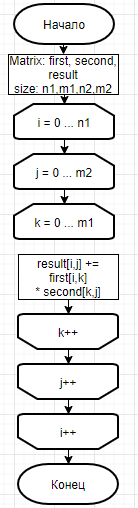
\includegraphics{Algorithm1.png}}
		\caption{Схема стандартного алгоритма умножения матриц}
		\label{Algorithm1}
	\end{figure}
	\newpage
	На \hyperref[Algorithm2]{ [\ref{Algorithm2}]} изображена схема алгоритма Винограда.
	\begin{figure}[h!]
		\center{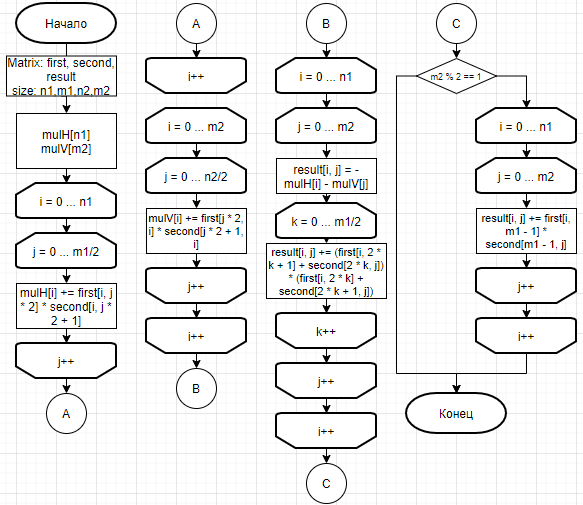
\includegraphics{Algorithm2.png}}
		\caption{Схема алгоритма Винограда}
		\label{Algorithm2}
	\end{figure}
	\newpage
	На \hyperref[Algorithm3]{рисунке  [\ref{Algorithm3}]} изображена схема модифицированного алгоритма Винограда.
	\begin{figure}[h!]
		\center{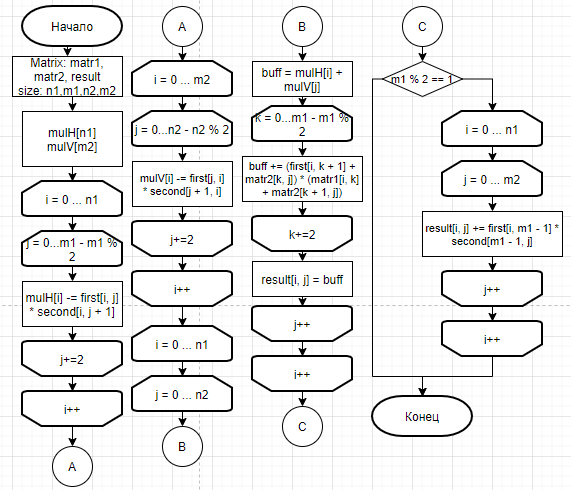
\includegraphics{Algorithm3.png}}
		\caption{Схема модифицированного алгоритма Винограда}
		\label{Algorithm3}
	\end{figure}
	\newpage
		 \subsection{Оценка трудоемкости}
		Модель трудоемкости для оценки алгоритмов:
		\newline
		Cтоимость базовых операций единица:
		\newline
		$=,+,*,<,>,<=,>=,==,!=,[],+=,-=,*=,/=,++,--$
		\newline
		\indent 
		\subsubsection{Трудоемкость стандартного алгоритма}
	     Трудоемкость внутреннего цикла N1= (8 + 2) * n2
		\newline
		Трудоемкость второго цикла N2 = (2 + 1 + N1) * m2 = (10*n2 + 3) * m2
		\newline
		Трудоемкость ввнешнего цикла N3 = (2 + 1 + N2) * n1 = (3 + (10*n2 + 3) * m2) * n1
		\newline
		Трудоемкость алгоритма = N3 + 1 = (3 + (10*n2 + 3) * m2) * n1 + 1 = 10*n2*m2*n1 + 3*m2*n1 + 3*n1 + 1
		\subsubsection{Трудоемкость алгоритма Винограда}
		Первый цикл: $\frac{15}{2}n_{1}m_{1}+5n_{1}+2$\\
		Второй цикл: $\frac{15}{2}m_{2}n_{2}+5m_{2}+2$\\
		Третий цикл: $13n_{1}m_{2}m_{1}+12n_{1}m_{2}+4n_{1}+2$\\
		Условный оператор: 
		\begin{equation}
		\begin{cases}
			2, \text{невыполнение} \\
			15n_{1}m_{2} + 4n_{1} + 2 , \text{выполнение}
		\end{cases}
		\end{equation}
		
		Результат:	$13n_{1}m_{2}m_{1}+\frac{15}{2}n_{1}m_{1}+\frac{15}{2}m_{2}n_{2}+12n_{1}m_{2}+5n_{1}+5m_{2}+4n_{1}+6+$\newline
				\begin{equation}	
		\begin{cases}
			2, \text{невыполнение}\\
			15n_{1}m_{2} + 4n_{1} + 2, \text{выполнение}\\
	\end{cases} 
	\end{equation}
		\subsubsection{Трудоемкость оптимизированого алгоритма Винограда}
			Первый цикл: $\frac{11}{2}n_{1}m_{1}+4n_{1}+2$\par
		Второй цикл: $\frac{11}{2}m_{2}n_{2}+4m_{2}+2$\par
		Третий цикл: $\frac{17}{2}n_{1}m_{2}m_{1}+9n_{1}m_{2}+4n_{1}+2$\newline
		Условный оператор: 
		\begin{equation}
		\begin{cases}
			2, \text{невыполнение}\\
			10n_{1}m_{2} + 4n_{1} + 2, \text{выполнение}\\
		\end{cases}
		\end{equation}
		\newline
		Результат:
		$\frac{17}{2}n_{1}m_{2}m_{1}+\frac{11}{2}n_{1}m_{1}+\frac{11}{2}m_{2}n_{2}+9n_{1}m_{2}+8n_{1}+4m_{2}+6+$\newline
		\begin{equation}
		\begin{cases}
			2, \text{невыполнение}\\
			10n_{1}m_{2} + 4n_{1} + 2, \text{выполнение}\\
		\end{cases}
		\end{equation}
		
	\newpage
	\subsection{Вывод}
	В данном разделе были рассмотрены схемы алгоритмов умножения матриц, была рассчитана трудоемкость алгоритмов и обозначены требования к ПО.
	
	\newpage
	\section{Технологическая часть}
	Ниже будут представлены средствы реализации и листинги реализованной программы.
	\subsection{Средcтва реализации}
	Выбранный язык программирования - С++, так как требований по конкретнему языку не выдвигалось и он был изучен во время обучения. Среда разработки - Visual Studio Code.\cite{vs-code}
	\newline
	\indent Функции вычисления процессорного времени - QueryPerfomanceCounter из библиотеки WinAPI.\cite{winapi}
	
	\subsection{Реализации алгоритмов}
	Ниже представлены листинги реализаций алгоритмов.
	На листинге \hyperref[stkkd]{[\ref{stkkd}]} представлен стандартный алгоритм умножения матриц.
	\begin{lstlisting}[label=stkkd, caption=Стандартный алгоритм умножения матриц]
	vector<vector<int>> multiplyClassic(vector< vector<int>> first, vector< vector<int>> second)
{
    int nFirst = first.size();
    int nSecond = second.size();
   
    vector<vector<int>> result;
    if (nFirst > 0 && nSecond > 0 && first[0].size() == nSecond && second[0].size() != 0)
    {
        int mSecond = second[0].size();

        result = createZeroMatrix(nFirst, mSecond);
        for (int i = 0; i < nFirst; i++)
        {
            for (int j = 0; j < mSecond; j++)
            {
                for (int k = 0; k < nSecond; k++)
                {
                    result[i][j] += first[i][k] * second[k][j];
                }
            }
        }
    }

    return result;
}
	\end{lstlisting}
		На листинге \hyperref[vin]{[\ref{vin}]} Представлен алгоритм Винограда.
	\begin{lstlisting}[label=vin,caption=Алгоритм Винограда]
	vector<vector<int>> multiplyVinograd(vector< vector<int>> first, vector< vector<int>> second)
{
    int nFirst = first.size();
    int nSecond = second.size();
   
    vector<vector<int>> result;

    if (nFirst > 0 && nSecond > 0 && first[0].size() == nSecond && second[0].size() != 0)
    {
        int mSecond = second[0].size();
        int mFirst = nSecond;

        result = createZeroMatrix(nFirst, mSecond);

        vector<int> mulH, mulV;
        mulH.reserve(nFirst);
        mulV.reserve(mSecond);

        for (int i = 0; i < nFirst; i++)
        {
            mulH[i] = 0;
            for (int j = 0; j < mFirst / 2; j++)
            {
                mulH[i] += first[i][j * 2] * first[i][j * 2 + 1];
            }
        }

        for (int i = 0; i < mSecond; i++)
        {
            mulV[i] = 0;
            for (int j = 0; j < nSecond / 2; j++)
            {
                mulV[i] += second[j * 2][i] * second[j * 2 + 1][i];
            }
        }

        for (int i = 0; i < nFirst; i++)
        {
            for (int j = 0; j < mSecond; j++)
            {
                result[i][j] = - mulH[i] - mulV[j];
                for (int k = 0; k < mFirst / 2; k++)
                {
                    result[i][j] += (first[i][2 * k + 1] + second[2 * k][j]) * (first[i][2 * k] + second[2 * k + 1][j]);
                }
            }
        }

        if (mFirst % 2 == 1)
        {
            for (int i = 0; i < nFirst; i++)
            {
                for (int j = 0; j < mSecond; j++)
                {
                    result[i][j] += first[i][mFirst - 1] * second[mFirst - 1][j];
                }
            }
        }
    }

    return result;
}
	\end{lstlisting}
		На листинге \hyperref[vinopt]{[\ref{vinopt}]} Представлен алгоритм Винограда оптимизированный.
	\begin{lstlisting}[label=vinopt,caption=Алгоритм Винограда оптимизированный]
	vector<vector<int>> multiplyVinogradOpt(vector< vector<int>> first, vector< vector<int>> second)
{
    int nFirst = first.size();
    int nSecond = second.size();
   
    vector<vector<int>> result;

    if (nFirst > 0 && nSecond > 0 && first[0].size() == nSecond && second[0].size() != 0)
    {
        int mSecond = second[0].size();
        int mFirst = nSecond;

        result = createZeroMatrix(nFirst, mSecond);

        vector<int> mulH, mulV;
        mulH.reserve(nFirst);
        mulV.reserve(mSecond);

        int m1Mod2 = mFirst % 2;
        int n2Mod2 = nSecond % 2;

        int temp = nSecond - n2Mod2;
        for (int i = 0; i < mSecond; i++)
        {
            mulV[i] = 0;
            for (int j = 0; j < temp; j += 2)
            {
                mulV[i] += second[j][i] * second[j + 1][i];
            }
        }

        temp = mFirst - m1Mod2;
        for (int i = 0; i < nFirst; i++)
        {
            mulH[i] = 0;
            for (int j = 0; j < temp; j += 2)
            {
                mulH[i] += first[i][j] * first[i][j + 1];
            }
        }

        for (int i = 0; i < nFirst; i++)
        {
            for (int j = 0; j < mSecond; j++)
            {
                int buff = - (mulH[i] + mulV[j]);
                for (int k = 0; k < temp; k += 2)
                {
                    buff += (first[i][k + 1] + second[k][j]) * (first[i][k] + second[k + 1][j]);
                }
                result[i][j] = buff;
            }
        }

        if (m1Mod2 == 1)
        {
            temp = mFirst - 1;
            for (int i = 0; i < nFirst; i++)
            {
                for (int j = 0; j < mSecond; j++)
                {
                    result[i][j] += first[i][temp] * second[temp][j];
                }
            }
        }
    }

    return result;
}
	\end{lstlisting}

	\subsection{Вывод}
	В данном разделе были описаны средства реализации, были представлены листинги реализации стандартного алгоритма умножения матриц, обычного и оптимизированного алгоритма Винограда.

	\newpage
	\section{Экспериментальная часть}
	В данной главе будут представлен пример работы программы, результат экспериментов по замеру времени и произведен сравнительный анализ алгоритмов по затрачиваемому времени.
	\subsection{Пример работы программы}
	Пример работы программы представлен на рисунке \hyperref[programmWork]{[\ref{programmWork}]}
	 	\begin{figure}[h!]
		 	\center{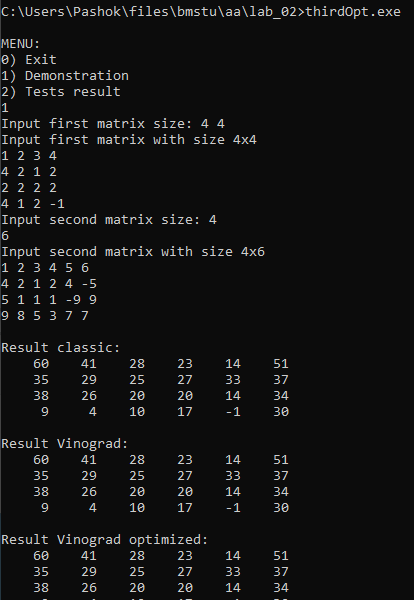
\includegraphics[scale=0.9]{programmWork.png}}
		 	\caption{Пример работы программы}
		 	\label{programmWork}
	 	\end{figure}
	
	\subsection{Сравнительный анализ алгоритмов по времени}
	Эксперименты проводятся на квадратных матрицах со стороной длиной от 2 до 252 с шагом 50 (результаты на рисунке \hyperref[resultShort]{[\ref{resultShort}]}
	\begin{figure}[h!]
		 	\center{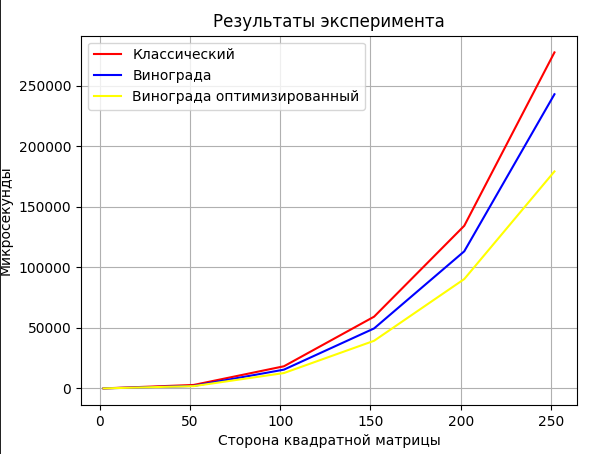
\includegraphics{resultShort.png}}
		 	\caption{Результаты на матрицах со стороной от 2 до 252}
		 	\label{resultShort}
	 	\end{figure}
	 	\newpage
	И на строках длины от 302 до 502 с шагом 50 (результаты на рисунке \hyperref[resultLong]{[\ref{resultLong}]}
	\begin{figure}[h!]
		 	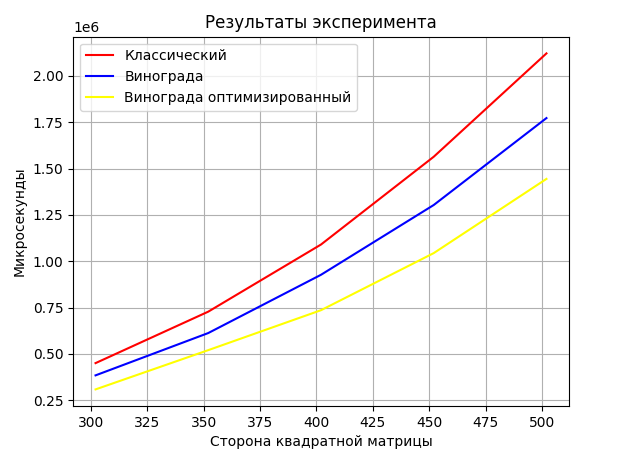
\includegraphics{resultLong.png}
		 	\caption{Результаты на матрицах со стороной от 302 до 502}
		 	\label{resultLong}
	 	\end{figure}
	 	\newpage
	 	\subsection{Вывод}
	Как видно из графиков, самым долгим алгоритмом является стандартный алгоритм. Самым быстрым является оптимизированный алгоритм Винограда. Простой алгоритм Винограда алгоритм быстрее стандартного, но уступает своей оптимизированной версииы.
	\newpage
	\begin{center}
		\section*{Заключение}
	\end{center}
	\addcontentsline{toc}{section}{Заключение}
	\indent \indent В данной лабораторной работе были изложены теоретические основы стандартного умножения матриц и алгоритма Винограда, они были разработаны и реализованы, были проведены эксперименты по замеру времени работы разработанных алгоритмов и проведены сравнения алгоритмов по результатам эксперимента. Также была дана оценка трудоемкости.
	\newpage
	\addcontentsline{toc}{section}{Список литературы}
	
	\begin{center}
	\begin{thebibliography}{3}
	\bibitem{vinogradRef}
	Умножение матриц [Электронный ресурс]. Режим доступа: (дата обращения - 02.10.2020) Свободный. URL: http://www.algolib.narod.ru/Math/Matrix.html
	\bibitem{vs-code}
	Visual Studio Code [Электронный ресурс]. Режим доступа: (дата обращения - 02.10.2020) Свободный. URL: code.visualstudio.com
	\bibitem{winapi}
		WinAPI. Функция QueryPerformanceCounter [Электронный ресурс]. Режим доступа: (дата обращения - 02.10.2020) Свободный. URL: https://docs.microsoft.com/en-us/windows/win32/api/profileapi/nf-profileapi-queryperformancecounter
	\end{thebibliography}
	\end{center}
\end{document}